\documentclass[acmlarge]{acmart}
\AtBeginDocument{%
  \providecommand\BibTeX{{%
    \normalfont B\kern-0.5em{\scshape i\kern-0.25em b}\kern-0.8em\TeX}}}

\usepackage{geometry} % see geometry.pdf on how to lay out the page. There's lots.
\usepackage{amsthm}
\usepackage{url}
% \geometry{a4paper} % or letter or a5paper or ... etc
% \geometry{landscape} % rotated page geometry

% See the ``Article customise'' template for come common customisations

\title{Survey of ZK-SNARK}
\author{Yuncong Zhang}
\authornotemark[1]
\email{yczhangsjtu@163.com}
\affiliation{%
  \institution{Shanghai Jiao Tong University}
  \streetaddress{Dongchuan Rd. 800}
  \city{Minhang}
  \state{Shanghai}
  \postcode{200240}
}

\newcommand{\Setup}{\mathsf{Setup}}
\newcommand{\Prove}{\mathsf{Prove}}
\newcommand{\Verify}{\mathsf{Verify}}
% \date{} % delete this line to display the current date

%%% BEGIN DOCUMENT
\begin{document}

% \tableofcontents
% \newpage
\begin{abstract}
\end{abstract}

\maketitle

\section{Introduction}

Zero-Knowledge Succinct Non-interactive ARgument of Knowledge (zkSNARK)~\cite{BitanskyCCT12} enables verifying computation outputs without knowing the inputs and faster than the original computation.
Currently, zkSNARKs are under active research, particularly due to their applications in blockchains~\cite{Ben-SassonCG0MTV14, SunALY17}, where zkSNARKs facilitate creating confidential transactions that conceal part or all of the transaction details.
Recent years have seen an explosion of zkSNARK implementations enjoying different properties, including constant-size proofs~\cite{Groth16, GennaroGP013, Ben-SassonCGTV13, ParnoHG013, Ben-SassonCTV13}, universal or trustless setups~\cite{GrothKMMM18, MallerBKM19, BunzFS20, Ben-SassonBHR18, Ben-SassonCRSVW19, AmesHIV17}, and post-quantum security~\cite{Ben-SassonBHR18, Ben-SassonCRSVW19}.


However, the rapid development of zkSNARK poses considerable challenges for researchers to keep up with the state-of-the-art.
Existing zkSNARK implementations rely on a large and growing number of underlying tools.
It is increasingly complicated to understand the complete toolset and uncover its full potential to construct more efficient and secure zkSNARKs.
It is also tricky to assess and compare existing schemes due to the high-dimensionality of measurement metrics, including efficiency, security, and functionality.
Existing studies trying to overview this field are oversimplifying and never tried to illustrate existing concrete implementations~\cite{ZKProof20, Nitulescu19, WalfishB15}.
A comprehensive survey of literature in zkSNARKs can serve as an anchor of knowledge in this field of research, provide an overview of the most significant ideas behind current implementations, and inspire new perspectives to understand zkSNARKs.

In this paper, we present a survey that overviews the current status of zkSNARKs.
First, we discuss the concepts that are necessary to understand the related literature.
Then we recall the history of zkSNARKs and examine the motivations and insights behind each major contribution.
Finally, we propose a framework for classifying and evaluating the zkSNARK implementations in terms of efficiency, functionality, expressiveness, infrastructure, building blocks, and security assumptions.
Using this framework, we reveal potential ways to leverage the existing tools and patterns to construct zkSNARKs with improved properties.

\section{Preliminaries}

\subsection{zkSNARK}

A zkSNARK is called \emph{preprocessing} if the $\Setup$ algorithm takes the circuit $C$ as input.
Fig.~\ref{fig:pp.zksnark} illustrates how preprocessing zkSNARK works.
\begin{figure}[ht!]
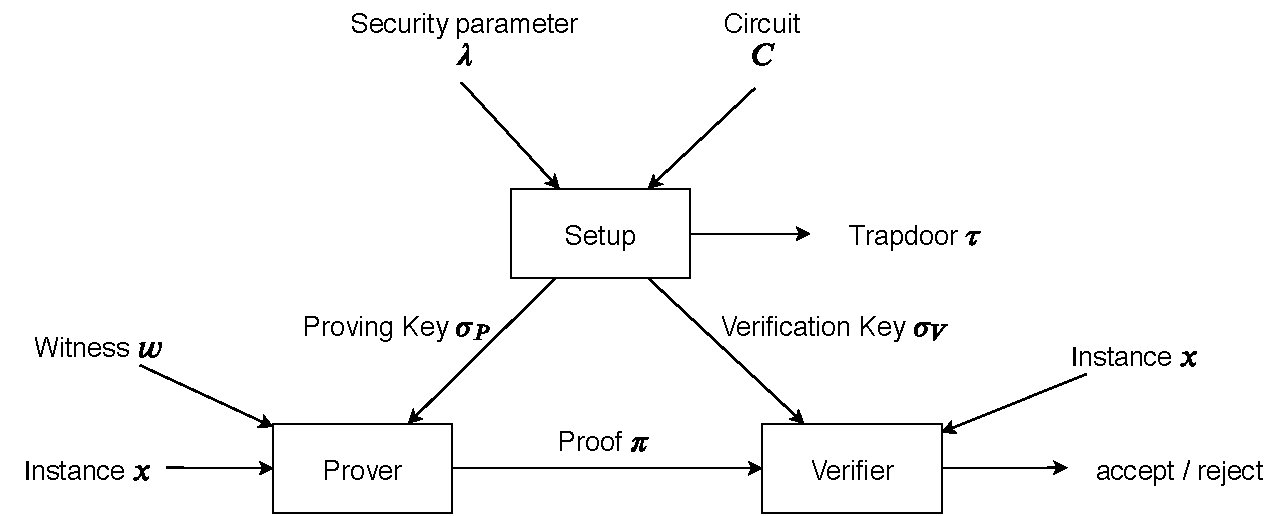
\includegraphics[width=0.8\textwidth]{images/ppzksnark.pdf}
\caption{Preprocessing zkSNARK}
\label{fig:pp.zksnark}
\descriptionlabel{
The $\Setup$ algorithm takes as inputs both the security parameter $\lambda$ and a circuit $C$, and outputs common reference strings, i.e. the proving key $\sigma_P$ and the verification key $\sigma_V$, to the prover and verifier respectively.
$\Setup$ also outputs a trapdoor $\tau$ which enables simulating proofs without witness.
The $\Prove$ algorithm takes as inputs an instance $x$ with corresponding witness $w$, together with proving key $\sigma_P$, and outputs the proof $\pi$ as validation of $x$.
The $\Verify$ algorithm verifies the correctness of $x$ with proof $\pi$ and verification key $\sigma_V$, and decides if to accept or reject.}
\Description{}
\end{figure}

\section{Efficiency}

In evaluating the efficiency of zkSNAKRs, the properties we care most about are proving time, verification time, proof sizes, and common reference string sizes.
Fig.~\ref{fig:snark.sizes} summarizes the asymptotic complexities of current zkSNARK implementations.
\begin{figure}[ht!]
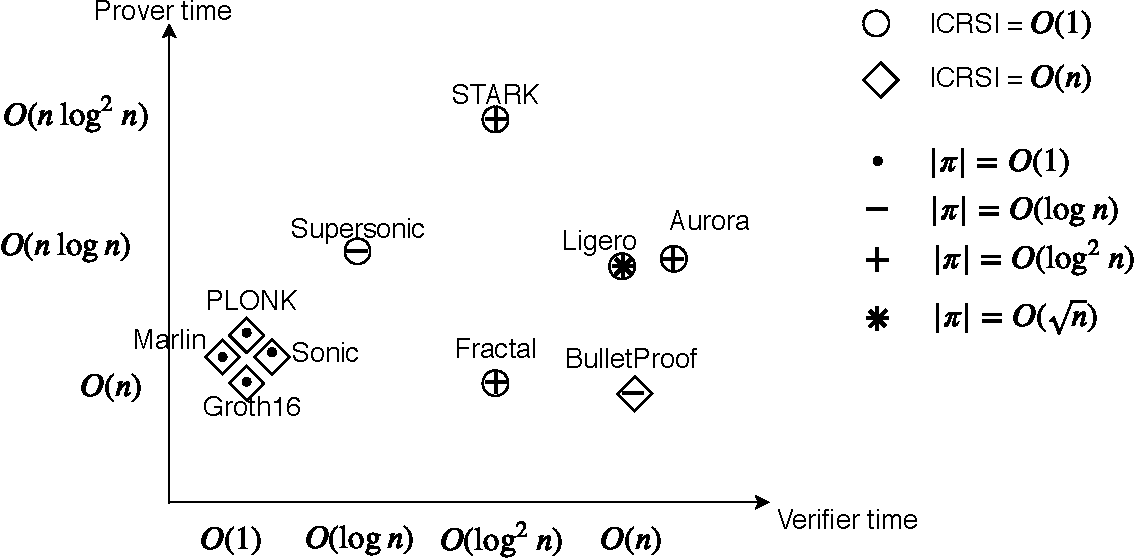
\includegraphics[width=0.8\textwidth]{images/snark-sizes.pdf}
\caption{Asymptotic complexities of zkSNARK implementations}
\label{fig:snark.sizes}
\descriptionlabel{
The big-$O$ notation here hides the security parameter $\lambda$.
The $n$ denotes the statement size.
For circuit-based zkSNARKs, $n$ is the circuit size.
For statements with succinct representation, e.g. STARK, $n$ is the length of execution trace, i.e. the size of the circuit representing the unrolled computation.}
\Description{}
\end{figure}


\bibliographystyle{unsrt}
\bibliography{reference}

\end{document}